\documentclass[11pt]{article}
    
    \usepackage{caption}
    \usepackage{graphicx}
    \usepackage{mathtools}
    \usepackage{bookmark}
    \graphicspath{ {img/} }
    \setlength{\parindent}{0pt}
    \DeclareCaptionType{equ}[][]
    \usepackage[svgnames]{xcolor}
    \graphicspath{ {./img/} }

    
    \newcommand*{\plogo}{\fbox{$\mathcal{BM}$}}
    
    \usepackage{PTSerif}
    
    \begin{document} 
        
    \begin{titlepage}
    
        \raggedleft
        
        \vspace*{\baselineskip}
        
        {\Large Bryan Melanson}
        
        \vspace*{0.167\textheight}
        
        \textbf{\LARGE How to Not Fail}\\[\baselineskip]
        
        {\textcolor{Red}{\Huge Computer Architecture}}\\[\baselineskip]
        
        {\Large \textit{While never going to class}}
        
        \vfill
        
        {\large Computer Engineering 2020 ~~\plogo}
        
        \vspace*{3\baselineskip}
    
    \end{titlepage}

    \pagebreak
    
%%%%%%%%%%%%%%%%%%%%%%%%%%%%%%%%%%%%%%%%%%%%%%%%%
    \pdfbookmark[section]{\contentsname}{toc}
    
    \tableofcontents

%%%%%%%%%%%%%%%%%%%%%%%%%%%%%%%%%%%%%%%%%%%%%%%%%

\section{Introduction}

\subsection{RISC}

\textbf{RISC} (Reduced Instruction Set Computer) is an architecture which allowed for the exploitation of instruction level parallelism and the use of caches. This increased performance couldn't be matched by other architectures, and Intel 80x86 was forced to translate its instructions into RISC-like form internally to adopt RISC innovations. In low-end applications, this has lead to RISC architecture like ARM becoming dominant.

\subsection{Dennard Scaling}

Power density was a constant for a given area of silicon, even as the number of transistors increased, due to their smalll dimension. This held up until a certain level in 2004, when the current and voltage levels could no longer ensure the dependability of integrated circuits.

\subsection{Multiple Processors}

The end of Dennard Scaling meant that improve performance more processors would be implemented, since single core chips would be inefficient with the increasing number of transistors. This meant that designs would no longer rely on \textbf{Instruction Level Parallelism}.

\subsection{Classes of Parallelism}

\begin{itemize}
    \item \textbf{Data Level Parallelism} - data items operated on at the same time
    \item \textbf{Task Level Parallelism} - tasks performed independently in parallel
\end{itemize}

\subsection{Application Parallelism}

\begin{itemize}
    \item \textbf{Instruction Level Parallelism} - exploits data-level using pipelining and speculative execution
    \item \textbf{Vector Archictectures} - exploits data-level parallelism using single instructions on a collection of data in parallel
    \item \textbf{Thread Level Parallelism} - data or task-level parallelism allowing for interaction between parallel threads
    \item \textbf{Request Level Parallelism} - parallelism between decoupled tasks
\end{itemize}

\subsection{Flynn's Taxonomy}

\begin{itemize}
    \item \textbf{Single Instruction Stream, Single Data Stream} - a single processor operates on sequential computation but can exploit ILP
    \item \textbf{Single Instruction Stream, Single Data Stream} - the same instruction executed by multiple processors, uses data level parallelism
    \item \textbf{Multiple Instruction Streams, Single Data Stream} - no implementation to date
    \item \textbf{Multiple Instruction Streams, Multiple Data Stream} - processesors have their own instructions and own data operated on, using task level parallelism. Used in warehouse level computing, exploiting request level parallelism where many independent tasks can proceed in parallel
\end{itemize}

\subsection{Warehouse Scale Computers}

Warehouse Scale Computers \textbf{WSC}s are collections of servers or \textbf{clusters} which Software as a Service (SaaS) uses as a single larger computer, capable of considerable processing power. Price-performance and power are critical.

\subsection{Instruction Set Architecture}

The old view of computer architecture focused on \textbf{Instruction Set Architecture} (ISA) design involves decisions regarding registers, memory addressing, addressing modes, instruction operands, available operations, control instructions and instruction encoding.\\

Computer architecture now involves specific requirementgs of the target machine, designs meant to maximize performance within constraints, ISA, microarchitecture, and requires consideration of how compilers work.

\subsection{RISC-V Instruction Formats}

\begin{center}
    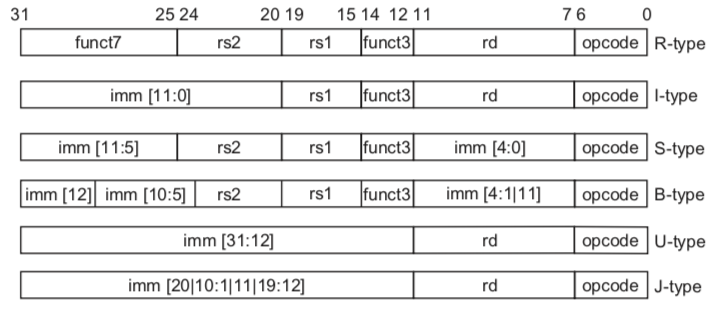
\includegraphics[scale=0.5]{riscv_formats}
\end{center}

\subsection{Latency and Bandwidth}

\subsection{Dynamic State Energy and Power}

\subsection{Die Yield}

\begin{center}
    \begin{equation}
    \text{Die Yield} = (1 + (\frac{\text{Defects/Area} \cdot \text{Area of Die}}{N}))^{-N}
    \end{equation}
\end{center}

\textbf{Die Yield} is a value which defines how likely it is that a die will be non-defective during the fabrication process. This value is a probability $< 1$, and the probability that a die will be defective is $1 - $Die Yield. \\
When converting between units of area (mm$^2$, cm$^2$), be sure to repeat conversion between units twice.

\begin{center}
    1 mm$^2$ = $\frac{1}{10 \text{cm}} \cdot \frac{1}{10 \text{cm}} = \frac{1}{100}$ cm$^2$
\end{center}

\subsection{Wafer Yield}

\textbf{Wafer Yield} is a value which describes how many dies (chips) can be created from a single wafer. This calculation is done using the size of a chip, and the diameter of each wafer. It takes into effect the square or rectangle shape of a chip and losses due to rounded sides of a wafer.

\begin{center}
\begin{equation} \text{Dies per wafer} = 
    \frac{\pi \cdot (\text{Wafer Diameter}/2)^2}{\text{Die area}} - \frac{\pi \cdot \text{Wafer diameter}}{\sqrt{2 \cdot \text{Die area}}}    
\end{equation}
\end{center}

These values can be used to calculate the cost of each die:

\begin{center}
    Cost of die = $\frac{\text{Cost of wafer}}{\text{Dies per wafer}\cdot\text{Die yield}}$
\end{center}

\subsection{Dependability}

\begin{itemize}
    \item Mean Time to Failure (MTTF)
    \item Mean Time to Repair (MTTR)
    \item Mean Time Between Failures (MTBF)
    \item Availability = MTTF / MTBF
\end{itemize}

\subsection{Performance}

\subsubsection{Execution Time}

\subsubsection{Speedup}

\subsubsection{Processor Performance Equation}

\end{document}
